\section{Introduction}

\begin{figure}[t!]
  \centering
  \subfloat[Current state-of-practice]{%
    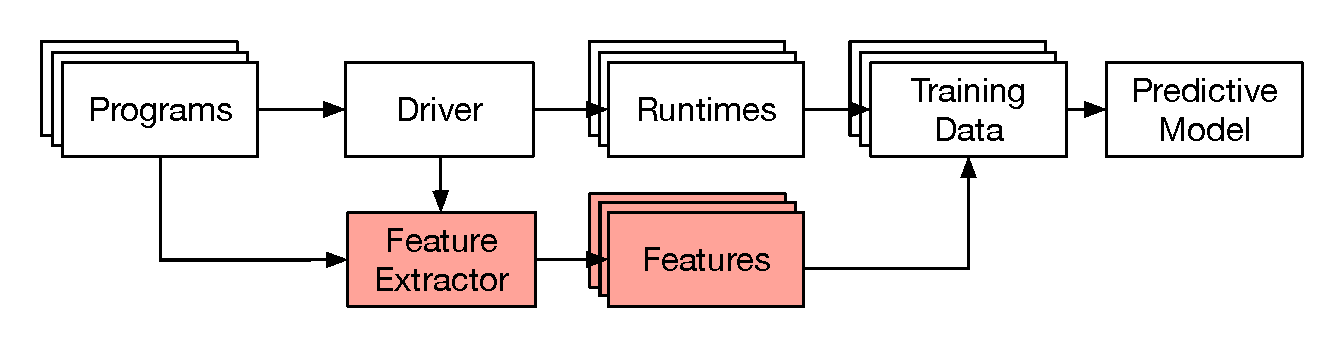
\includegraphics[width=.95\columnwidth]{img/training_model_a}%
    \label{fig:overview-a}%
  }\\*%
  \subfloat[The proposed approach]{%
    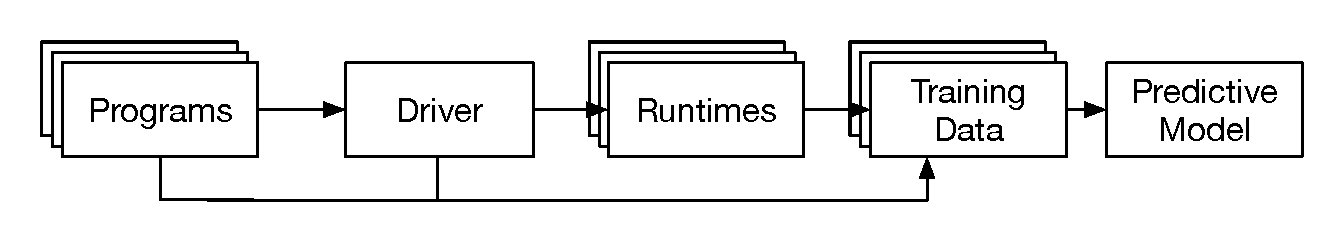
\includegraphics[width=.95\columnwidth]{img/training_model_b}%
    \label{fig:overview-b}%
  }%
  \caption[Building a predictive model]{%
    Building a predictive model. The model is originally trained on performance
    data and features extracted from the source code and the runtime behaviour.
    We propose bypassing feature extraction, instead learning directly over raw
    program source code.%
  }%
  \label{fig:overview}
\end{figure}


There are countless scenarios during the compilation and execution of a parallel program where decisions must be made as to how, or if, a particular optimization should be applied. Modern compilers and runtimes are rife with hand coded \emph{heuristics} which perform this decision making. The performance of parallel programs is thus dependent on the quality of these heuristics.

Hand-written heuristics require expert knowledge, take a lot of time to construct, and in many cases lead to suboptimal decisions. Researchers have focused on machine learning as a means to constructing high quality heuristics that often outperform their handcrafted equivalents~\cite{Micolet2016,Falch2015,Stephenson2005,Agakov,Cummins2015a}. A \emph{predictive model} is trained, using supervised machine learning, on empirical performance data and important quantifiable properties, or \emph{features}, of representative programs. The model learns the correlation between these features and the optimization decision that maximizes performance. The learned correlations are used to predict the best optimization decisions for new programs. Previous works in this area were able to build machine learning based heuristics with less effort, that outperform ones created manually experts~\cite{Grewe2013,Magni2014}.

Still, experts are not completely removed from the design process, which is shown in Figure~\ref{fig:overview-a}. Selecting the appropriate features is a manual undertaking which requires a deep understanding of the system. The designer essentially decides which compile or runtime characteristics affect optimization decisions and expresses them in ways that make it easy to model their relationship to performance. Failing to identify an important feature has a negative effect on the resulting heuristic. For example, in~\cite{Cummins2017a} the authors discovered that~\cite{Grewe2013} did not identify one such feature, causing performance to be 40\% lower on average.

To make heuristic construction fast and cheap, we must take humans out of the loop. While techniques for automatic feature generation from the compiler IR have been proposed in the past~\cite{Namolaru2010a,Leather2014}, they do not solve the problem in a practical way. They are deeply embedded into the compiler, require expert knowledge to guide the generation, have to be repeated from scratch for every new heuristic, and their search time can be prohibitive. Our insight was that such costly approaches are not necessary any more. Deep learning techniques have shown astounding successes in identifying complex patterns and relationships in images~\cite{Krizhevsky2012,He2016}, audio~\cite{Lee2009b}, and even computer code~\cite{Allamanis2014,Allamanis2014a}. We hypothesized that deep neural networks should be able to automatically extract features from source code. Our experiments showed that even this was a conservative target: with deep neural networks we can bypass static feature extraction and learn optimization heuristics directly on raw code.

Figure~\ref{fig:overview-b} shows our proposed methodology. Instead of manually extracting features from input programs to generate training data, program code is used directly in the training data. Programs are fed through a series of neural networks which learn how code correlates with performance. Internally and without prior knowledge, the networks construct complex abstractions of the input program characteristics and correlations between those abstractions and performance. Our work replaces the need for compile-time or static code features, merging feature and heuristic construction into a single process of joint learning. Our system admits auxiliary features to describe information unavailable at compile time, such as the sizes of runtime input parameters. Beyond these optional inclusions, we are able to learn optimization heuristics without human guidance.

By employing \emph{transfer learning}~\cite{Yosinski2014}, our approach is able to produce high quality heuristics even when learning on a small number of programs. The properties of the raw code that are abstracted by the beginning layers of our neural networks are mostly independent of the optimization problem. We reuse these parts of the network across heuristics, and, in the process, we speed up learning considerably.

We evaluated our approach on two problems: heterogeneous device mapping and GPU thread coarsening. Good heuristics for these two problems are important for extracting performance from heterogeneous systems, and the fact that machine learning has been used before for heuristic construction for these problems allows direct comparison. Prior machine learning approaches resulted in good heuristics which extracted 73\% and 79\% of the available performance respectively but required extensive human effort to select the appropriate features. Nevertheless, our approach was able to outperform them by 14\% and 12\%, which indicates a better identification of important program characteristics, without any expert help. We make the following contributions:
%
\begin{itemize}
  \item We present a methodology for building compiler heuristics without any need for feature engineering.
  \item A novel tool DeepTune for automatically constructing optimization heuristics without features. DeepTune outperforms existing state-of-the-art predictive models by 14\% and 12\% in two challenging optimization domains.
  \item We apply, for the first time, \emph{transfer learning} on compile-time and runtime optimizations, improving the heuristics by reusing training information across different optimization problems, even if they are unrelated.
\end{itemize}
